% Created 2021-01-24 Sun 22:49
% Intended LaTeX compiler: pdflatex
\documentclass[11pt]{article}
\usepackage[utf8]{inputenc}
\usepackage[T1]{fontenc}
\usepackage{graphicx}
\usepackage{grffile}
\usepackage{longtable}
\usepackage{wrapfig}
\usepackage{rotating}
\usepackage[normalem]{ulem}
\usepackage{amsmath}
\usepackage{textcomp}
\usepackage{amssymb}
\usepackage{capt-of}
\usepackage{hyperref}
\usepackage{minted}
\hypersetup{colorlinks=true, linkcolor=black, filecolor=red, urlcolor=blue}
\usepackage[turkish]{babel}
\author{Eren Hatırnaz}
\date{3 Şubat 2020}
\title{Yazılım Gündemi - 2020/05\\\medskip
\large 27 Ocak - 2 Şubat 2020}
\hypersetup{
 pdfauthor={Eren Hatırnaz},
 pdftitle={Yazılım Gündemi - 2020/05},
 pdfkeywords={},
 pdfsubject={},
 pdfcreator={Emacs 27.1 (Org mode 9.3)},
 pdflang={Turkish}}
\begin{document}

\maketitle
\tableofcontents \clearpage\shorthandoff{=}

\begin{center}
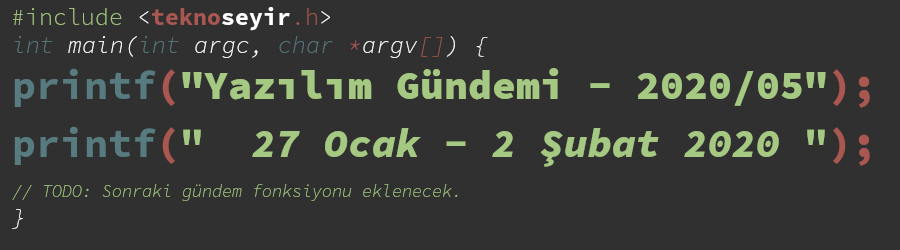
\includegraphics[width=.9\linewidth]{gorseller/yazilim-gundemi-banner.png}
\end{center}

\begin{center}
\href{../04/yazilim-gundemi-2020-04.pdf}{< Önceki Gündem} | \textbf{27 Ocak - 2 Şubat 2020} | \href{../06/yazilim-gundemi-2020-06.pdf}{Sonraki Gündem >}

\href{https://teknoseyir.com/blog/yazilim-gundemi-2020-05}{TeknoSeyir'de Oku}
\end{center}

\section{CWA, Teknoloji ve Oyun sektörü çalışanlarını \href{https://gizmodo.com/cwa-launches-new-effort-to-unionize-game-and-tech-worke-1840861878}{örgütlemek istiyor}}
\label{sec:org3470f54}
Amerika'daki büyük işçi sendikalarından biri olan \href{https://en.wikipedia.org/wiki/Communications\_Workers\_of\_America}{The Communications Workers
of America}, şimdi de teknoloji ve oyun sektörü çalışanlarını bünyesine katmak
ve onların da sorunlarını dile getirmek için paçaları sıvadı. Bu sendika
hakkında pek bir bilgim yok ama bu haber özelinde konuşmak istediklerim olduğu
için gündeme aldım bunu.

Örgütlü mücadele her zaman için ilgili sektördeki sorunların dile
getirilebilmesi ve çözüme ulaştırılabilmesi açısından en iyi yöntemlerden
birisidir. Konuyla ilgili atasözünün de dediği gibi: "Bir elin nesi var, iki
elin sesi var". Ülkemizde maalesef pek fazla iyi örneklerine rastlayamasak da
internet kullanıcıları olarak hepimizi etkileyen Adil Kullanım Noktası'nın
(AKN) kaldırılması olayının arkasında örgütlü bir mücadele var: \href{https://internettekalite.com/}{İnternette
Kalite Hareketi}. Bu minvalde yazılım geliştirme sektörü olarak da
sorunlarımızı dile getirebileceğimiz, çözüm yolları için uğraşlar
verebileceğimiz sendikalara ya da meslek örgütlerine ihtiyacımız var ve
ilerlediğimiz gelecekte bu ihtiyacın daha da çok olacağını düşünüyorum.
Ayrımcılıklar, fazla çalışma saatleri ve düşük ücretler, mobbing gibi sorunlar
hemen her sektörde karşımıza çıksa da, etik olmayan uygulamalar (şirketin
kullanıcıların verilerini izni olmadan kullanması vb.) ve hükumetlerle yapılan
anlaşmalar gibi sektörümüze özel sorunlar da mevcut.

Türkiye'de benim bildiğim kadarıyla bizim alanımızı kapsayan meslek örgütü
olarak \href{https://www.bmo.org.tr/}{Bilgisayar Mühendisleri Odası} var. Faaliyetleri hakkında pek fazla
bilgim olmasa da \href{https://www.bmo.org.tr/2020/01/23/mebin-teknik-liselerde-yazilim-egitimi-yontemi-cagdisidir/}{Delphi eğitimi protokolü için bildiri}yle farkına vardığım bir
oluşum oldu. Aslında önceden de ismini duymuştum fakat pek bakma fırsatım
olmamıştı. Sayfalarını incelediğimde "\href{https://www.bmo.org.tr/en-az-ucret/}{En Az Ücret Tanımları}" sayfası dikkatimi
çekti. BMO, 2018 yılından beri her yıl "Mühendislik Asgari Ücreti"
belirliyorlarmış. 2020 yılı için belirlenen Mühendislik Asgari Ücreti ise
5.000TL imiş. Sektöre ne kadar etkisi vardır bilinmez ama ben yine de bu tarz
örgütlü faaliyetlerin olması gerektiğini düşünüyorum. Mesleki standartların
belirlenmesi, haklarımızı aramak ve talep etmek için bu tarz örgütlere üye
olmakta ve aktif görev almakta fayda var. Ben de şahsen işe girdiğimde BMO'ya
üye olmayı düşünüyorum.

Bu konu hakkında siz ne düşünüyorsunuz? Sizce teknoloji sektörü çalışanları
olarak nasıl örgütlenmeliyiz? Haklarımızı nasıl aramalıyız? Yorumlar bölümünde
konuşalım.
\section{Cloudflare: "\href{https://blog.cloudflare.com/javascript-libraries-are-almost-never-updated/}{JavaScript kütüphaneleri projeye eklendikten sonra neredeyse hiç güncellenmiyor}"}
\label{sec:org13fde77}
Dünya çapında bir çok yerde veri merkezinin olması dolayısıyla CDN hizmetini
de çok kolay verebilen \href{https://www.cloudflare.com/}{Cloudflare} firması, bu hafta alt hizmeti olan \href{https://cdnjs.com/}{CDNJS} ile
ilgili bir analiz yayınladı. Bu analiz tam olarak bu haberin başlığındaki
cümleyi içeriyor. Yani geliştiriciler olarak bir JavaScript kütüphanesini bir
kere projeye ekliyoruz sonra güncellemelerle pek ilgilenmiyoruz.

\begin{figure}[htbp]
\centering
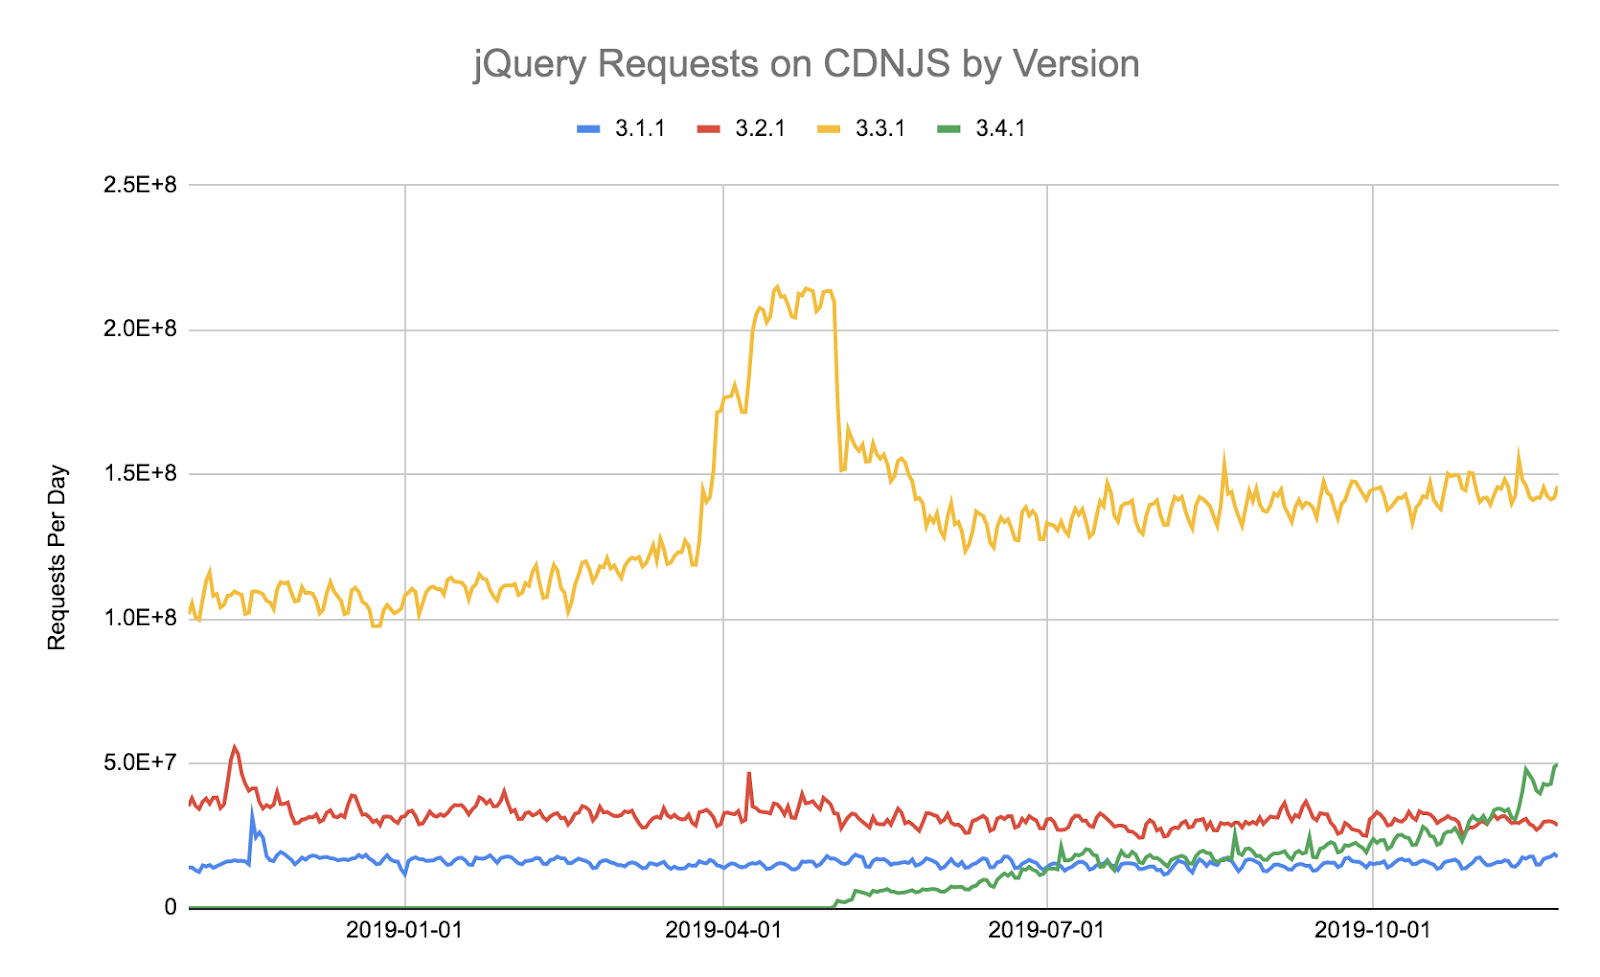
\includegraphics[width=.9\linewidth]{gorseller/cloudflare-jquery-1.png}
\caption{CDNJS sunucusuna bir günde gelen istek sayısına göre jQuery sürümleri grafiği}
\end{figure}

Grafikte sizin de kolayca görebileceğiniz üzere Mayıs 2019 ayında jQuery'nin
yeni versiyonu olan 3.4.1 çıkmış olmasına rağmen diğer eski sürümlerin
popülaritesini düşürememiş. En çok istek alan jQuery sürümü ise 3.3.1 olmuş.

\begin{figure}[htbp]
\centering
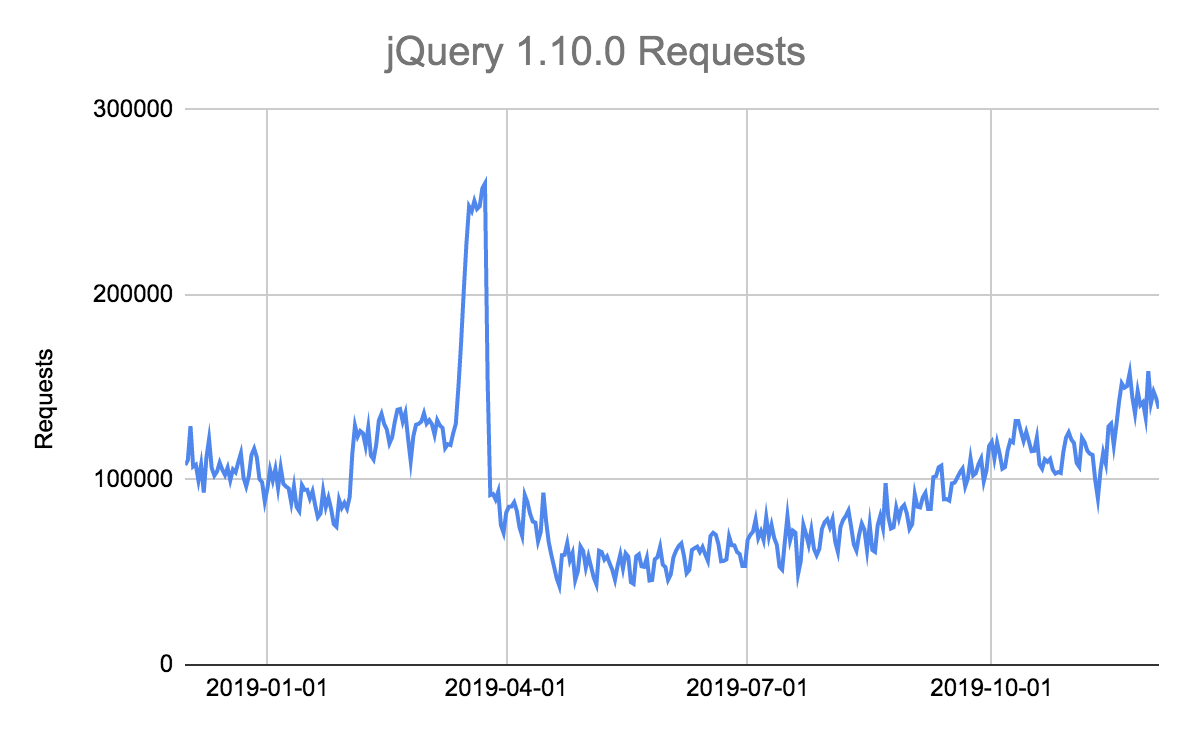
\includegraphics[width=.9\linewidth]{gorseller/cloudflare-jquery-2.png}
\caption{Hatta 2013 yılında yayınlanan jQuery 1.10.0 sürümü bile hata hatırı sayılır derecede istek alıyor}
\end{figure}

Elbette sisteminiz ilgili sürümlerde sorunsuz çalışıyorsa ve ihtiyaçlarınızı
karşılıyorsa bir üst sürüme geçmek için efor sarf etmenize gerek yok
("çalışıyorsa dokunma") ama yine de güvenlik açıkları vb. nedenlerden dolayı
projenize eklediğiniz her bağımlılığın sürümlerini takibe almakta fayda var.
\section{GitHub, illegal Instagram-API \href{https://github.com/github/dmca/blob/master/2020/01/2020-01-22-facebook.md}{deposunu kilitledi}}
\label{sec:org8518c2a}
\begin{figure}[htbp]
\centering
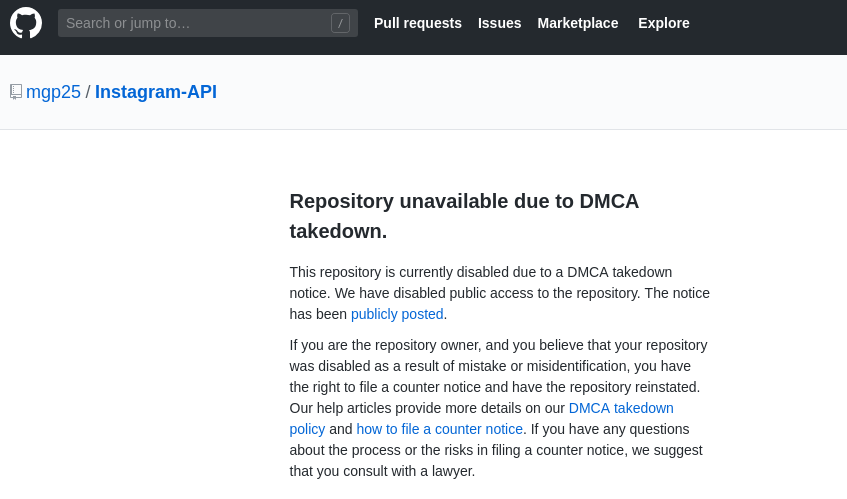
\includegraphics[width=.9\linewidth]{gorseller/github-instagram-api.png}
\caption{İlgili \href{https://github.com/mgp25/Instagram-API}{GitHub sayfası}na girince sizi karşılayan sayfa}
\end{figure}

Instagram platformunun resmi olarak biz geliştiricilere sunduğu bir API
sistemi olmadığı için çoğu kişi GitHub'da Mgp25 nickli kullanıcının
yayınladığı resmi olmayan, PHP ile yazıldığını hatırladığım (yanlış hatırlıyor
da olabilirim) Instagram-API isimli kütüphaneyi kullanıyordu. Fakat geçtiğimiz
hafta (bu hafta gündem oldu) GitHub, Facebook'un isteği doğrultusunda bu
GitHub deposunu kilitledi. Artık deponun sayfasına girmeye çalıştığınızda sizi
yukarıdaki ekran görüntüsündeki gibi bir açıklama karşılıyor (bu durum deponun
forkları için de geçerli). Açıkcası kullanım amacı kişiden kişiye değişiklik
gösterse de çoğu kişi bu kütüphaneyi maalesef beğenme ve takip etme botları
gibi amaçlar için kullandığından ve bazı telif hakkı sorunlarına yol açtığı
için Facebook'u pek de haksız bulmuyorum.

Yapılan işlemlerle ilgili daha detaylı ve hukuki bilgiler için konu başlığına
eklediğim bağlantıya bakabilirsiniz.
\section{Qt 2020 yılına \href{https://www.qt.io/blog/qt-offering-changes-2020}{değişikliklerle girdi}}
\label{sec:org01204b4}
Popüler platformlar-arası (cross-platform) uygulama geliştirme
framework'lerinden olan Qt, bu hafta bloglarında yayınladıkları yazı ile
fiyatlandırma ve lisanslamayla ilgili değişikliklere gittiklerini duyurdular.
Maalesef değişiklikler pek bizim açımızdan olumlu yönde değil. Şöyle ki:

\begin{itemize}
\item Artık Qt binary'lerini indirmek için Qt hesabınız olması gerek.
\item Uzun-dönem destekli (LTS - Long-term-supported) sürümler ve çevrimdışı
kurumlar (offline installer) artık sadece ticari lisans sahiplerine
sunulacak.
\item Startuplar ve küçük ölçekli şirketler için Qt fiyatlandırması yıllık \$499
oldu.
\end{itemize}

Yayınladıkları blog yazısında elbette tüm bu değişiklikler için mantıklı
sebepler bulduklarını iddia ediyorlar. Örneğin ilk maddeyi şöyle savunmuşlar.
Qt açık kaynak kullanıcılarının bile artık Qt binary indirmesi için "Qt
Account" açması gerekiyor. Çünkü bu şekilde kendilerinin servislerini en iyi
şekilde kullanabilecek ve katkı sağlayabilecekmişiz. Ayrıca bu sayede hata
raporları, forumlar, kod incelemeleri vb birçok şeye de erişebilecekmişiz.
Kısaca "kimler qt indiriyor ve kullanıyor elimizde tam listesi olsun
istiyoruz" demiyorlar da lafı dolandırıyorlar işte. Qt açık kaynağı
kodlarından derleyip kullanabilirsiniz tabii ki ama kolay olsun direkt binary
indireyim derseniz "Qt Account" şart.

LTS sürümlerinin ve çevrimdışı kurulumların da sadece ticari lisans
sahiplerine verilmesini de açık kaynak kullanıcıların yeni sürümlere daha iyi
adapte olabilmesi için yapıyoruz demişler ama kendilerinin de açıkladığı gibi
asıl mesele iş modellerini değiştirmek istemeler ve ticari lisansı firmalar
için daha cazip kılmak istemeleri. Bunu biraz anlayışla karşılayabiliyorum
çünkü ticari bir şirket oldukları için bu tarz kaygıları olması normal.

Kısaca haberi özetleyecek olursak Qt, açık kaynak kullanıcıları için biraz
vanayı kısıyor. Açık kaynak kullanıcıları için kötü haber maalesef. Neyse, en
azından tamamen ücretli hale gelmedi.
\section{Go 1.15 sürümü için \href{https://blog.golang.org/go1.15-proposals}{planlar yapıldı}}
\label{sec:org6fc8bb1}
Go programlama dili gün geçtikçe gelişmeye ve sürüm atlamaya devam ediyor. Bu
hafta yayınladıkları blog yazısı ile Go takımı Şubat ayı içerisinde bir
aksilik olmazsa, şu an beta sürecinde olan 1.14 sürümünü RC1 etiketi ile
yayınlayacaklarını duyurmuşlar. Aynı zamanda bir sonraki sürüm olan 1.15 için de
bazı kararların verilmesine başlamışlar. Bu yılın Ağustos ayında yayınlanması
planlanan bu sürüm üzerinde çalışmak için GitHub üzerinden gelen şu üç öneriyi
seçmişler:

\begin{itemize}
\item \href{https://golang.org/issue/32479}{\#32479}: Diagnose string(int) conversion in \texttt{go vet}.
\item \href{https://golang.org/issue/4483}{\#4483}: Diagnose impossible interface-interface type assertions in \texttt{go vet}.
\item \href{https://golang.org/issue/28591}{\#28591}. Constant-evaluate index and slice expressions with constant strings
and indices.
\end{itemize}

Görüldüğü üzere daha çok Go dilinin komut satırı aracı olan \texttt{go vet} üzerine
odaklanmışlar gibi gözüküyor. \texttt{go vet} aracı vermiş olduğunuz .go uzantılı
dosyayı inceliyor ve duruma göre size hata ve uyarı veriyor. Her ne kadar
planlar aşağı yukarı yapılmış gibi gözükse de Go takımı 1.14 sürümünün
yayınlanmasından biraz sonra geliştirmeye başlayacağı için 1.15 sürümü için
tartışmalara katılabilir ve yeni önerilerde bulunabilirsiniz. Henüz kapı tam
kapanmamış yani anlayacağız.

Üzerinde çalışılması planlanan özelliklerin ve sürecin detayları için konu
başlığına eklediğim blog yazısına bakabilirsiniz.
\section{RStudio, \href{https://blog.rstudio.com/2020/01/29/rstudio-pbc/}{Kamu Yararına Şirket oldu}}
\label{sec:org1da847d}
\href{https://www.r-project.org/}{R programlama dili} her ne kadar sektörel yazılımlarda pek tercih edilmese de
veri bilimi ve özellikle de istatistik alanında çalışan akademisyenlerin
gözdesi olmuş durumda. Çoğumuz R dilinin IDE'si sayılabilecek \href{https://rstudio.com/}{RStudio}
yazılımını aslında dilin bir parçası sanıyoruz. Hatta ben de bu haberle
karşılaşana kadar öyle sanıyordum fakat RStudio aslında ayrıca geliştirilen
bir araç, hatta şirketmiş. İşte bu şirket, bu hafta bloglarında yayınladıkları
yazı ile birlikte bir "\href{https://en.wikipedia.org/wiki/Public-benefit\_corporation}{Public Benefit Corparation} (PBC - Kamu Yararına
Şirket)" haline gelmiş. Sanırım Türkiye'de olmayan bir şirket türü, biraz
detaylarını araştırmaya çalıştım ama pek fazla bir şey anladığım söylenemez.
Yine de bizim alanımızla ilgili bir yazılım üreten bir şirketin dönüşmesi
olduğu için gündeme almak istedim.

Bundan sonraki ilerleyecekleri yolla ilgili detaylı bilgilere konu başlığına
eklediğim bağlantıyı inceleyebilirsiniz.
\section{Google App Maker \href{https://support.google.com/a/answer/9682494?hl=en}{hizmetini kapatıyor}}
\label{sec:org47d2ae0}
Gün geçmiyor ki Google bir ürününü ya da hizmetini \href{https://killedbygoogle.com/}{Google Mezarlığı}na
göndermesin. Bu hafta da G Suite isimli işletmeler için çeşitli hazır çözümler
içeren paketin içerisindeki App Maker hizmetini kapacağını duyurdu. İsminden
anladığım kadarıyla işletmeler için kod yazmadan basit mobil uygulamalar
oluşturmaya yarayan bir hizmetti. Geçtiğimiz haftalardaki bir yazılım gündemi
yazısının (bkz: \href{../03/yazilim-gundemi-2020-03.pdf}{Yazılım Gündemi - 2020/03}) "Diğer Haberler" bölümünde
Google'ın, kod yazmadan uygulama geliştirme aracı olan AppSheet'i satın
aldığını yazmıştım. Dolayısıyla böyle bir gelişme bizim için pek sürpriz
olmadı.

Bu hizmeti hemen kapatmıyorlar tabii ki ama ufaktan fişini çekmeye
hazırlanıyorlar. Süreç bu şekilde ilerleyecekmiş:

\begin{itemize}
\item \textbf{27 Ocak 2020}: Var olan uygulamalar çalışmaya devam edecek fakat App Maker
hizmetinin geliştirilmesine devam edilmeyecek. Kritik hatalar hâlâ mevcut.
\item \textbf{15 Nisan 2020}: Geliştiriciler bu tarihten itibaren yeni App Maker
uygulaması oluşturamayacaklar.
\item \textbf{19 Ocak 2021}: Var olan uygulamalar çalışmayacak. App Maker verileriniz
Cloud SQL üzerinde değişmeden duracak ve Google Cloud Platform
hesabınızının poliçelerini takip etmeye devam edecek. Son cümleyi ben de
tam anlamadım fakat sanırım GCP kapsamında bazı ücretlendirmeler fatura
edilebilir demek istiyorlar.
\end{itemize}

Yani anlayacağız Google yeni satın aldığı bir şirketin çözümünü kendi
sistemine entegre ediyor ve kendi çözümünü de kullanımdan kaldırıyor. Dağdan
gelen bağdakini kovdu yani. Konu başlığına eklediğim bağlantıda da zaten
Google, App Maker alternatifi olarak AppSheet'i göstermiş ve oraya geçilmesini
tavsiye etmiş. Eğer sistemi kullanıyorsanız konu başlığındaki bağlantıyı
mutlaka okuyun ve aksiyon almaya başlayın.
\section{Ekosistem ve topluluk anketleri}
\label{sec:orgcdd1d16}
\subsection{\href{https://surveys.jetbrains.com/s3/developer-ecosystem-survey-2020-sh}{JetBrains Developer Ecosystem Survey 2020}}
\label{sec:orgda3e9e3}
\begin{center}
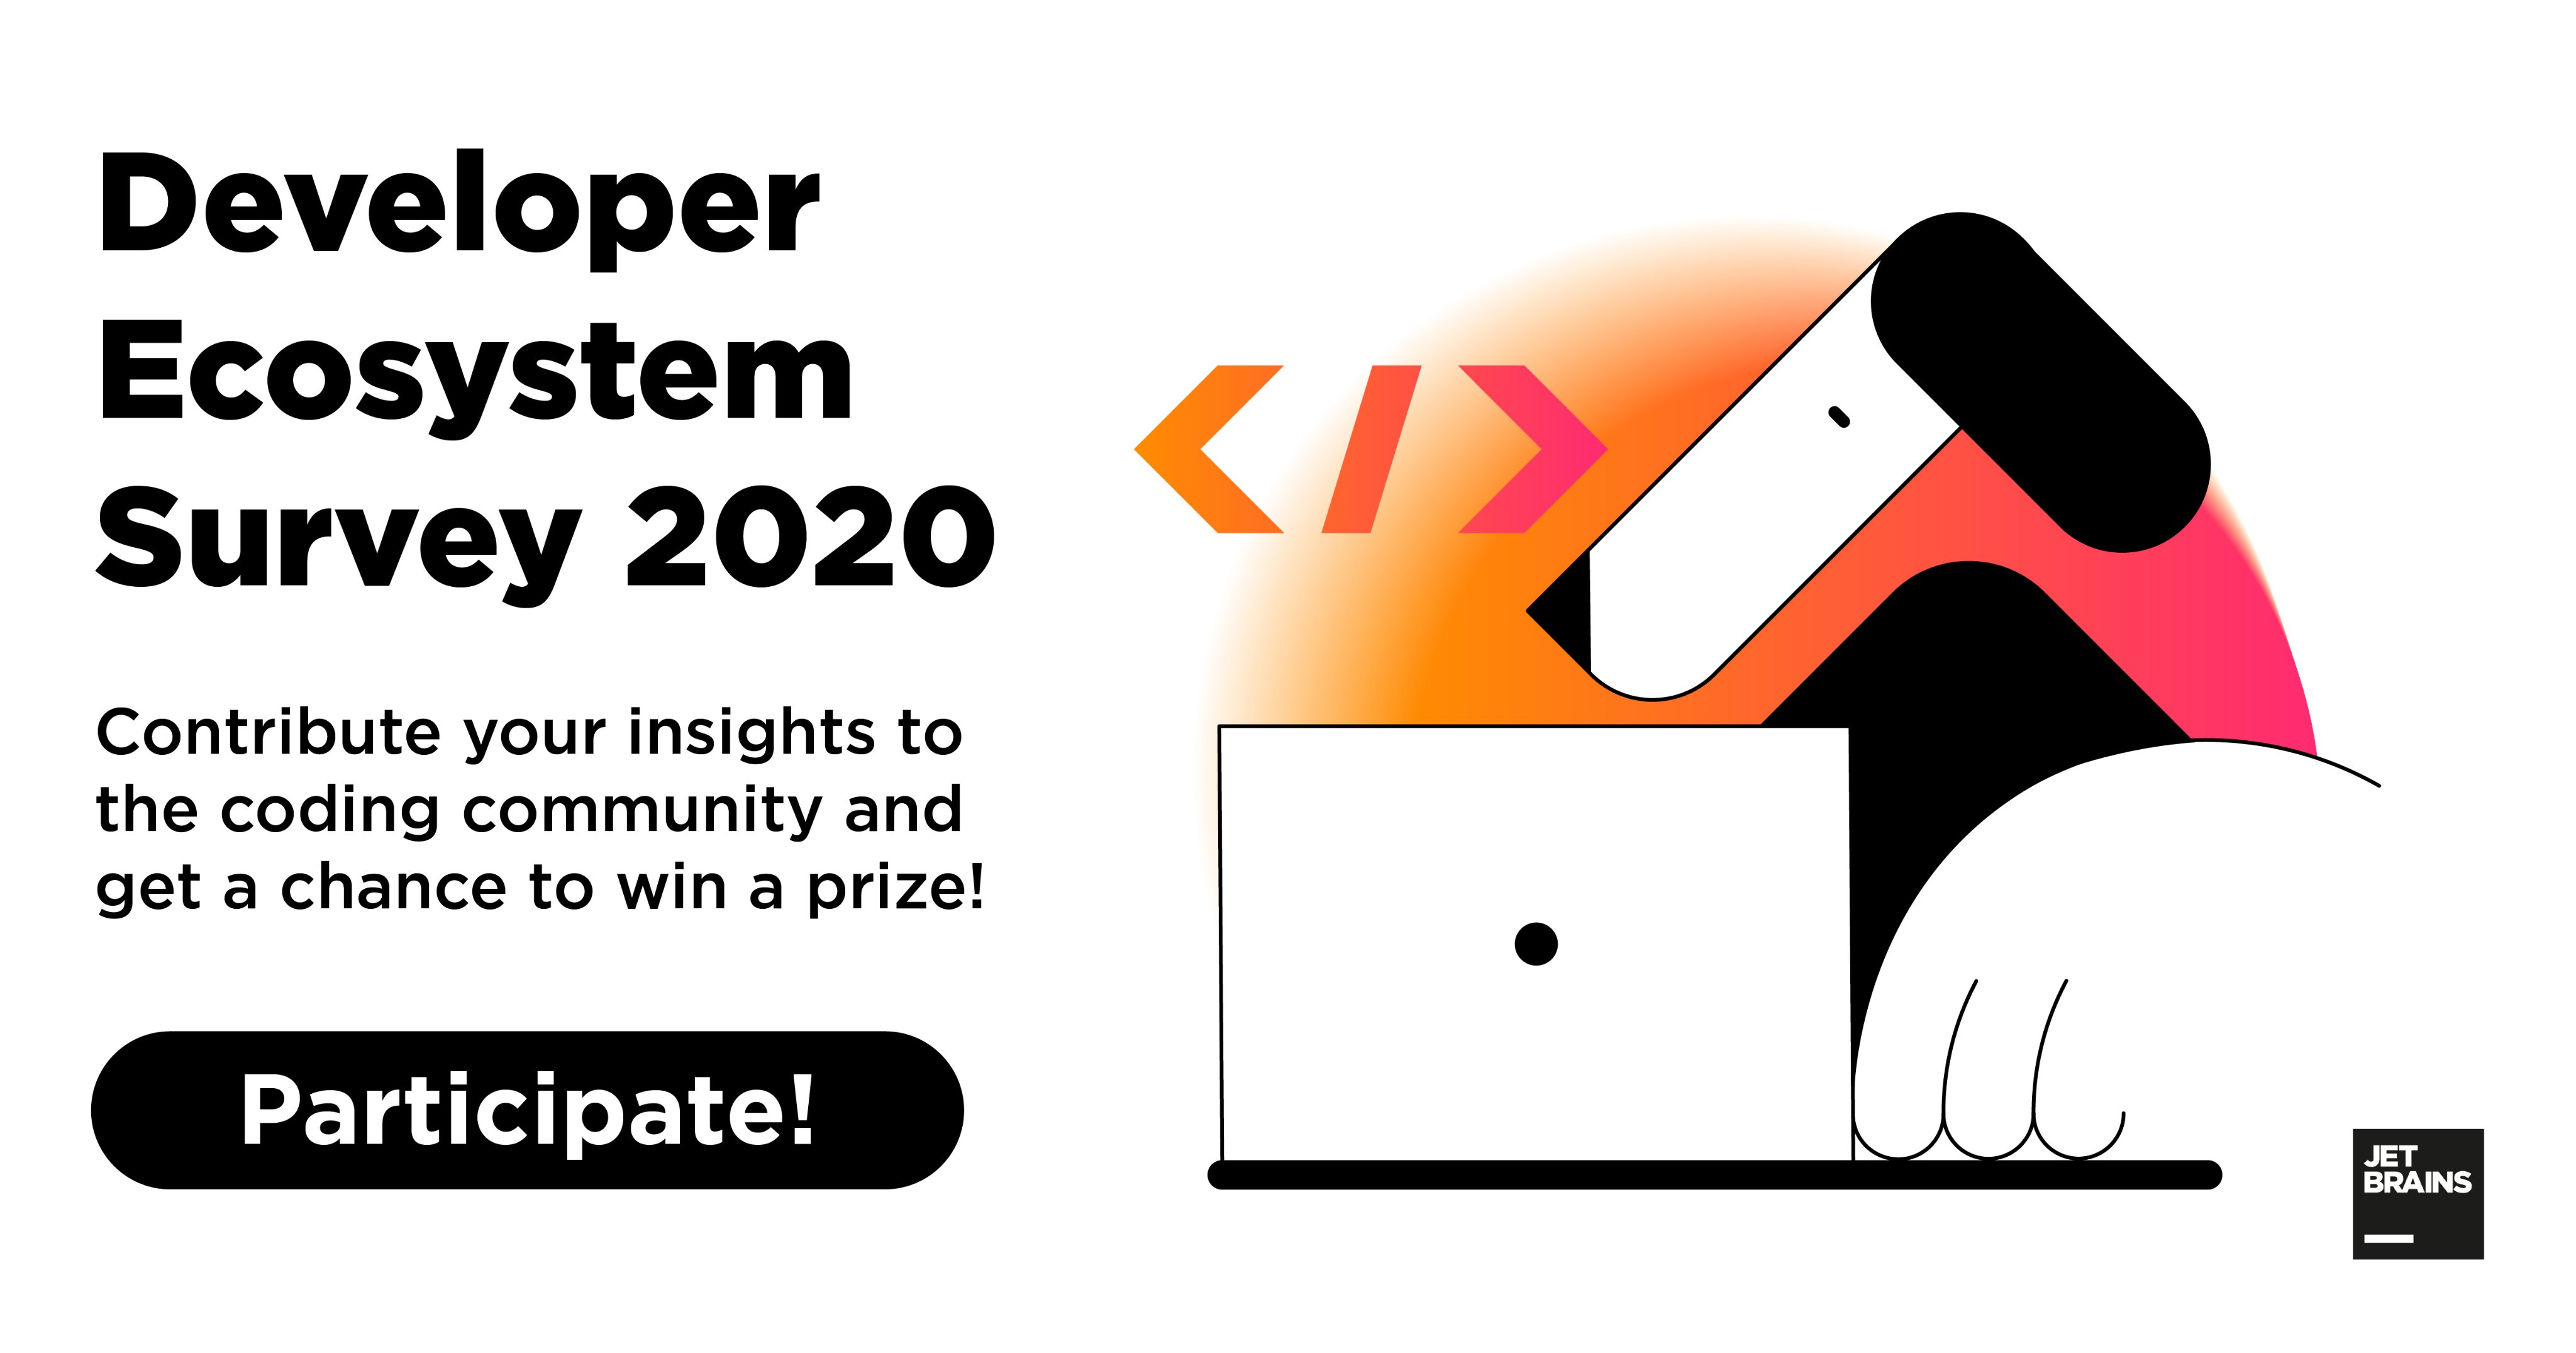
\includegraphics[width=.9\linewidth]{gorseller/jetbrains-anket.png}
\end{center}

JetBrains'in her yıl düzenli olarak yaptığı geliştirici ekosistemi anketi bu
yılda katılıma açıldı. Diğer anketlerden farklı olaran JetBrains'in ekonomik
gücü olduğu için katılımcılardan rastgele kişilere ödüller de (MacBook Pro,
\$300'lık Amazon hediye kartı ve JetBrains Sürpriz Hediye Paketi) veriyor. Ben
nasıl olsa çıkmaz diyerek MacBook Pro'yu seçtim. Anket biraz uzun 20-25
dakika sürebiliyor ama isterseniz kaydedip sonra da kaldığınız yerden
doldurmaya devam edebiliyorsunuz. Geçtiğimiz senenin anket sonuçları için:
\href{https://www.jetbrains.com/lp/devecosystem-2019/}{The State of Developer Ecosystem 2019}.
\subsection{\href{https://docs.google.com/forms/d/e/1FAIpQLSf-DvTpaz4oSPDMghdpHutdoY1Pn\_YqVa8JRLV2tPIiQcM3BA/viewform}{Yazılım Geliştiricileri Maaş Anketi 2020}}
\label{sec:orgedb69be}
\begin{center}
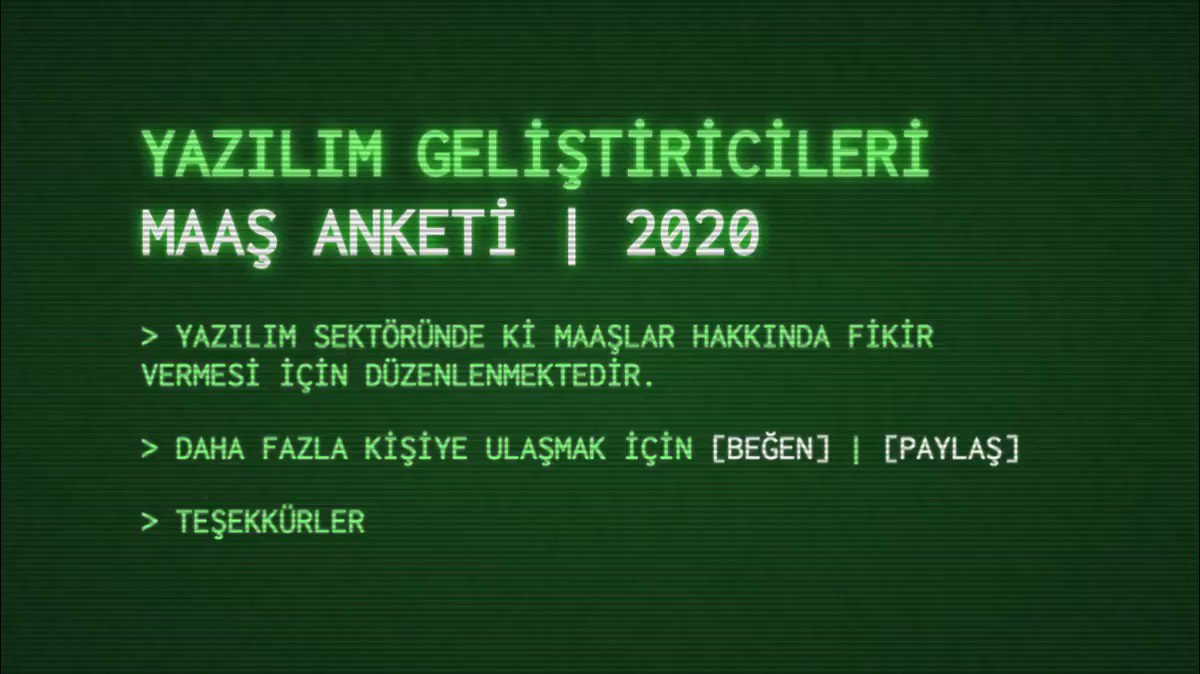
\includegraphics[width=.9\linewidth]{gorseller/yazilim-gelistirici-maas-anketi.png}
\end{center}

Twitter'daki \href{https://twitter.com/oncekiyazilimci}{oncekiyazilimci} nickli parodi hesabının 2 yıldır düzenli olarak
yaptığı bir anket çalışması. Ankete katılım 31 Mart 2020 tarihine kadar devam
edecekmiş. Önceki yılların anket sonuçları için bu sayfaları ziyaret
edebilirsiniz:
\begin{itemize}
\item \href{https://medium.com/@oncekiyazilimci/yaz\%C4\%B1l\%C4\%B1mc\%C4\%B1-maa\%C5\%9Flar\%C4\%B1-2019-f0e535d736a3}{Yazılımcı Maaşları | 2019}
\item \href{https://medium.com/@oncekiyazilimci/yaz\%C4\%B1l\%C4\%B1mc\%C4\%B1-maa\%C5\%9Flar\%C4\%B1-c312a05df5a6}{Yazılımcı Maaşları | 2018}
\end{itemize}
\section{Yaklaşan Etkinlikler}
\label{sec:org1b44425}
\begin{longtable}{|p{8cm}|l|l|}
\hline
Etkinlik İsmi & Yeri & Tarihi\\
\hline
\endfirsthead
\multicolumn{3}{l}{Önceki sayfadan devam ediyor} \\
\hline

Etkinlik İsmi & Yeri & Tarihi \\

\hline
\endhead
\hline\multicolumn{3}{r}{Devamı sonraki sayfada} \\
\endfoot
\endlastfoot
\hline
\href{https://www.meetup.com/Istanbul-Spring-Meetup/events/267716831/}{Spring Boot uygulamalarında derin Elasticsearch kullanımı} & İstanbul & 3 Şubat 19:00\\
\href{https://www.meetup.com/trendyol/events/267805404/}{Cloud Native Uygulamalarda GitLab + CI ile GitOps Pratikleri} & İstanbul & 4 Şubat 19:00\\
\href{https://www.meetup.com/python-istanbul/events/268319431/}{Python Saati 101 - The Zen of Software Developer} & İstanbul & 4 Şubat 19:00\\
\href{https://www.meetup.com/GDG-Cloud-Istanbul/events/268195069/}{Google Cloud Days 3 - Production-Scale ML Platform on GCP} & İstanbul & 5 Şubat 18:30\\
\href{https://kommunity.com/kodluyoruz/events/kanser-tedavisinde-derin-ogrenme-yontemlerinin-kullanimi}{Kanser Tedavisinde Derin Öğrenme Yöntemlerinin Kullanımı} & İstanbul & 6 Şubat 18:30\\
\href{https://www.meetup.com/IBMCloudTR/events/268323729/}{Watson ile Kendi Chatbot'unuzu Nasıl Oluşturursunuz?} & İstanbul & 6 Şubat 19:00\\
\href{https://www.meetup.com/TestHive/events/268357425/}{Test Automation Project With Spring Framework} & İstanbul & 11 Şubat 19:00\\
\href{https://www.meetup.com/Mekansal-Zeka/events/267511327/}{Mobil Harita Üretimi, HD-map ve Mekansal Zeka} & İstanbul & 13 Şubat 18:30\\
\href{https://www.meetup.com/Istanbul-Java-User-Group/events/267929475/}{RxJava'yı legacy koda uygulamak} & İstanbul & 13 Şubat 19:00\\
\href{https://www.meetup.com/ING-\%25C4\%25B0novasyon-Merkezi/events/268406663/}{Yapay Zeka Okuryazarlığı} & İstanbul & 14 Şubat 18:30\\
\href{https://www.meetup.com/Akademi-4-0/events/268053643/}{Makine Öğrenmesine Giriş - 101} & İstanbul & 15 Şubat 08:30\\
\href{https://kommunity.com/istanbulphp/events/microservices}{Microservices} & İstanbul & 15 Şubat 13:00\\
\href{https://www.meetup.com/GDGAnkara/events/268384563/}{Python ile Programlamaya Giriş} & Ankara & 15 Şubat 11:00\\
\hline
\end{longtable}
\section{Diğer Haberler}
\label{sec:org983e0cc}
\begin{itemize}
\item \href{https://openai.com/}{OpenAI} ve \href{https://pytorch.org/}{PyTorch} güçlerini \href{https://venturebeat.com/2020/01/30/openai-facebook-pytorch-google-tensorflow/}{birleştiriyor}.
\item Google, \href{https://tinygo.org/}{TinyGo} projesine \href{https://mobile.twitter.com/TinyGolang/status/1223887654158307328}{sponsor oldu}.
\item GitLab'ın Mercurial destekli fork'u açık kaynak ve özgür yazılım \href{https://heptapod.net/a-public-heptapod-for-free-and-open-source-software.html}{olarak
duyuruldu}: \href{https://heptapod.net/}{Heptapod}.
\item Rust programlama dilinin 1.41.0 \href{https://blog.rust-lang.org/2020/01/30/Rust-1.41.0.html}{sürümü duyuruldu}.
\item Rust takımı IDE dostu derleyicisini \href{https://www.infoq.com/news/2020/01/rust-analyser-ide-support/}{duyurdu}: \href{https://rust-analyzer.github.io/}{Rust Analyzer}.
\item GNU C kütüphanesinin 2.31 \href{https://lists.gnu.org/archive/html/info-gnu/2020-02/msg00001.html}{sürümü yayınlandı}.
\item Elixir programlama dilinin 1.10 \href{https://elixir-lang.org/blog/2020/01/27/elixir-v1-10-0-released/}{sürümü yayınlandı}.
\item JetBrains, \href{https://ktor.io/}{Ktor} framework sisteminin 1.3 \href{https://blog.jetbrains.com/kotlin/2020/01/ktor-1-3-release/}{sürümünü yayınladı}.
\item Google, Dagger kütüphanesinin 2.26 \href{https://github.com/google/dagger/releases/tag/dagger-2.26}{sürümünü yayınladı}.
\item \href{https://edgedb.com/}{EdgeDB} veritabanının 1.0 Alpha 2 \href{https://edgedb.com/blog/edgedb-1-0-alpha-2/}{sürümü duyuruldu}.
\item Dağıtık veritabanı sistemi \href{https://etcd.io/}{etcd}, 3.4.3 \href{https://etcd.io/blog/jepsen-343-results/}{sürümünü yayınladı}.
\item Unity oyun motorunun 2019.3 \href{https://blogs.unity3d.com/2020/01/28/unity-2019-3-is-now-available/}{sürümü duyuruldu}.
\item Godot oyun motorunun 3.2 \href{https://godotengine.org/article/here-comes-godot-3-2}{sürümü duyuruldu}.
\item Raspberry Pi'ye Vulkan \href{https://www.raspberrypi.org/blog/vulkan-raspberry-pi-first-triangle/}{desteği geliyor}.
\item Derin öğrenme kütüphanesi \href{https://github.com/explosion/thinc}{Thinc}, v8.0.0a0 \href{https://github.com/explosion/thinc/releases/tag/v8.0.0a0}{sürümünü yayınladı}.
\item Görsel bir şekilde Python kodu debug etmeye yarayan \href{https://github.com/CCExtractor/vardbg}{vardbg} aracının v0.11.6
\href{https://github.com/CCExtractor/vardbg/releases/tag/v0.11.6}{sürümü yayınlandı}.
\item Python veri analizi kütüphanesi \href{https://pandas.pydata.org/pandas-docs/stable/index.html}{Pandas}, 1.0.0 \href{https://pandas.pydata.org/pandas-docs/stable/whatsnew/v1.0.0.html}{sürümünü yayınladı}. \href{https://github.com/pandas-dev/pandas}{GitHub
Deposu}
\item OpenAPIGenerator v4.2.3 \href{https://github.com/OpenAPITools/openapi-generator/releases/tag/v4.2.3}{çıktı}.
\end{itemize}
\section{Lisans}
\label{sec:org4805d84}
\begin{center}
\begin{center}

\includegraphics[height=1.5cm]{../../../img/CC_BY-NC-SA_4.0.png}
\end{center}

\href{yazilim-gundemi-2020-05.pdf}{Yazılım Gündemi - 2020/05} yazısı \href{https://erenhatirnaz.github.io}{Eren Hatırnaz} tarafından \href{http://creativecommons.org/licenses/by-nc-sa/4.0/}{Creative Commons
Atıf-GayriTicari-AynıLisanslaPaylaş 4.0 Uluslararası Lisansı} (CC BY-NC-SA 4.0)
ile lisanslanmıştır.
\end{center}
\end{document}
